% Template for PLoS
% Version 3.5 March 2018
%
% % % % % % % % % % % % % % % % % % % % % %
%
% -- IMPORTANT NOTE
%
% This template contains comments intended 
% to minimize problems and delays during our production 
% process. Please follow the template instructions
% whenever possible.
%
% % % % % % % % % % % % % % % % % % % % % % % 
%
% Once your paper is accepted for publication, 
% PLEASE REMOVE ALL TRACKED CHANGES in this file 
% and leave only the final text of your manuscript. 
% PLOS recommends the use of latexdiff to track changes during review, as this will help to maintain a clean tex file.
% Visit https://www.ctan.org/pkg/latexdiff?lang=en for info or contact us at latex@plos.org.
%
%
% There are no restrictions on package use within the LaTeX files except that 
% no packages listed in the template may be deleted.
%
% Please do not include colors or graphics in the text.
%
% The manuscript LaTeX source should be contained within a single file (do not use \input, \externaldocument, or similar commands).
%
% % % % % % % % % % % % % % % % % % % % % % %
%
% -- FIGURES AND TABLES
%
% Please include tables/figure captions directly after the paragraph where they are first cited in the text.
%
% DO NOT INCLUDE GRAPHICS IN YOUR MANUSCRIPT
% - Figures should be uploaded separately from your manuscript file. 
% - Figures generated using LaTeX should be extracted and removed from the PDF before submission. 
% - Figures containing multiple panels/subfigures must be combined into one image file before submission.
% For figure citations, please use "Fig" instead of "Figure".
% See http://journals.plos.org/plosone/s/figures for PLOS figure guidelines.
%
% Tables should be cell-based and may not contain:
% - spacing/line breaks within cells to alter layout or alignment
% - do not nest tabular environments (no tabular environments within tabular environments)
% - no graphics or colored text (cell background color/shading OK)
% See http://journals.plos.org/plosone/s/tables for table guidelines.
%
% For tables that exceed the width of the text column, use the adjustwidth environment as illustrated in the example table in text below.
%
% % % % % % % % % % % % % % % % % % % % % % % %
%
% -- EQUATIONS, MATH SYMBOLS, SUBSCRIPTS, AND SUPERSCRIPTS
%
% IMPORTANT
% Below are a few tips to help format your equations and other special characters according to our specifications. For more tips to help reduce the possibility of formatting errors during conversion, please see our LaTeX guidelines at http://journals.plos.org/plosone/s/latex
%
% For inline equations, please be sure to include all portions of an equation in the math environment.  For example, x$^2$ is incorrect; this should be formatted as $x^2$ (or $\mathrm{x}^2$ if the romanized font is desired).
%
% Do not include text that is not math in the math environment. For example, CO2 should be written as CO\textsubscript{2} instead of CO$_2$.
%
% Please add line breaks to long display equations when possible in order to fit size of the column. 
%
% For inline equations, please do not include punctuation (commas, etc) within the math environment unless this is part of the equation.
%
% When adding superscript or subscripts outside of brackets/braces, please group using {}.  For example, change "[U(D,E,\gamma)]^2" to "{[U(D,E,\gamma)]}^2". 
%
% Do not use \cal for caligraphic font.  Instead, use \mathcal{}
%
% % % % % % % % % % % % % % % % % % % % % % % % 
%
% Please contact latex@plos.org with any questions.
%
% % % % % % % % % % % % % % % % % % % % % % % %

\documentclass[10pt,letterpaper]{article}
\usepackage[top=0.85in,left=2.75in,footskip=0.75in]{geometry}

% amsmath and amssymb packages, useful for mathematical formulas and symbols
\usepackage{amsmath,amssymb}

% Use adjustwidth environment to exceed column width (see example table in text)
\usepackage{changepage}

% Use Unicode characters when possible
\usepackage[utf8x]{inputenc}

% textcomp package and marvosym package for additional characters
\usepackage{textcomp,marvosym}

% cite package, to clean up citations in the main text. Do not remove.
\usepackage{cite}

% Use nameref to cite supporting information files (see Supporting Information section for more info)
\usepackage{nameref,hyperref}

% line numbers
\usepackage[right]{lineno}

% ligatures disabled
\usepackage{microtype}
\DisableLigatures[f]{encoding = *, family = * }

% color can be used to apply background shading to table cells only
\usepackage[table]{xcolor}

% array package and thick rules for tables
\usepackage{array}

% create "+" rule type for thick vertical lines
\newcolumntype{+}{!{\vrule width 2pt}}

% create \thickcline for thick horizontal lines of variable length
\newlength\savedwidth
\newcommand\thickcline[1]{%
  \noalign{\global\savedwidth\arrayrulewidth\global\arrayrulewidth 2pt}%
  \cline{#1}%
  \noalign{\vskip\arrayrulewidth}%
  \noalign{\global\arrayrulewidth\savedwidth}%
}

% \thickhline command for thick horizontal lines that span the table
\newcommand\thickhline{\noalign{\global\savedwidth\arrayrulewidth\global\arrayrulewidth 2pt}%
\hline
\noalign{\global\arrayrulewidth\savedwidth}}


% Remove comment for double spacing
%\usepackage{setspace} 
%\doublespacing

% Text layout
\raggedright
\setlength{\parindent}{0.5cm}
\textwidth 5.25in 
\textheight 8.75in

% Bold the 'Figure #' in the caption and separate it from the title/caption with a period
% Captions will be left justified
\usepackage[aboveskip=1pt,labelfont=bf,labelsep=period,justification=raggedright,singlelinecheck=off]{caption}
\renewcommand{\figurename}{Fig}

% Use the PLoS provided BiBTeX style
\bibliographystyle{plos2015}

% Remove brackets from numbering in List of References
\makeatletter
\renewcommand{\@biblabel}[1]{\quad#1.}
\makeatother



% Header and Footer with logo
\usepackage{lastpage,fancyhdr,graphicx}
\usepackage{epstopdf}
%\pagestyle{myheadings}
\pagestyle{fancy}
\fancyhf{}
%\setlength{\headheight}{27.023pt}
%\lhead{
\includegraphics[width=2.0in]{PLOS-submission.eps}}
\rfoot{\thepage/\pageref{LastPage}}
\renewcommand{\headrulewidth}{0pt}
\renewcommand{\footrule}{\hrule height 2pt \vspace{2mm}}
\fancyheadoffset[L]{2.25in}
\fancyfootoffset[L]{2.25in}
\lfoot{\today}

%% Include all macros below

\newcommand{\lorem}{{\bf LOREM}}
\newcommand{\ipsum}{{\bf IPSUM}}

%% END MACROS SECTION

\newcommand{\grace}[1]{\textcolor{blue}{#1}}
\newcommand{\ruchi}[1]{\textcolor{red}{#1}}
\newcommand{\sticky}{proglobular~}
\usepackage{makecell}

\renewcommand\theadalign{bc}
\renewcommand\theadfont{\bfseries}
\renewcommand\theadgape{\Gape[4pt]}
\renewcommand\cellgape{\Gape[4pt]}


\begin{document}
\vspace*{0.2in}

% Title must be 250 characters or less.
\begin{flushleft}
{\Large
\textbf\newline{Sequence specificity despite intrinsic disorder: how a disease-associated  Val/Met polymorphism shifts tertiary interactions in a long disordered protein} % Please use "sentence case" for title and headings (capitalize only the first word in a title (or heading), the first word in a subtitle (or subheading), and any proper nouns).
}
\newline
% Insert author names, affiliations and corresponding author email (do not include titles, positions, or degrees).
\\
Ruchi Lohia\textsuperscript{1},
Reza Salari\textsuperscript{1},
Grace Brannigan\textsuperscript{1,2*},
\\
\bigskip
\textbf{1} Center for Computational and Integrative Biology, Rutgers University, Camden, NJ, USA
\\
\textbf{2} Department of Physics, Rutgers University, Camden, NJ, USA
\\
\bigskip

% Insert additional author notes using the symbols described below. Insert symbol callouts after author names as necessary.
% 
% Remove or comment out the author notes below if they aren't used.
%
% Primary Equal Contribution Note
%\Yinyang These authors contributed equally to this work.

% Additional Equal Contribution Note
% Also use this double-dagger symbol for special authorship notes, such as senior authorship.
%\ddag These authors also contributed equally to this work.

% Current address notes
%\textcurrency Current Address: Dept/Program/Center, Institution Name, City, State, Country % change symbol to "\textcurrency a" if more than one current address note
% \textcurrency b Insert second current address 
% \textcurrency c Insert third current address

% Deceased author note
%\dag Deceased

% Group/Consortium Author Note
%\textpilcrow Membership list can be found in the Acknowledgments section.

% Use the asterisk to denote corresponding authorship and provide email address in note below.
* grace.brannigan@rutgers.edu(GB)

\end{flushleft}

\renewcommand{\thepage}{S\arabic{page}}  
\renewcommand{\thesection}{S\arabic{section}}   
\renewcommand{\thetable}{S\arabic{table}}   
\renewcommand{\figurename}{}
\renewcommand{\thefigure}{S\arabic{figure} Fig}

\clearpage
\begin{figure}[!ht]
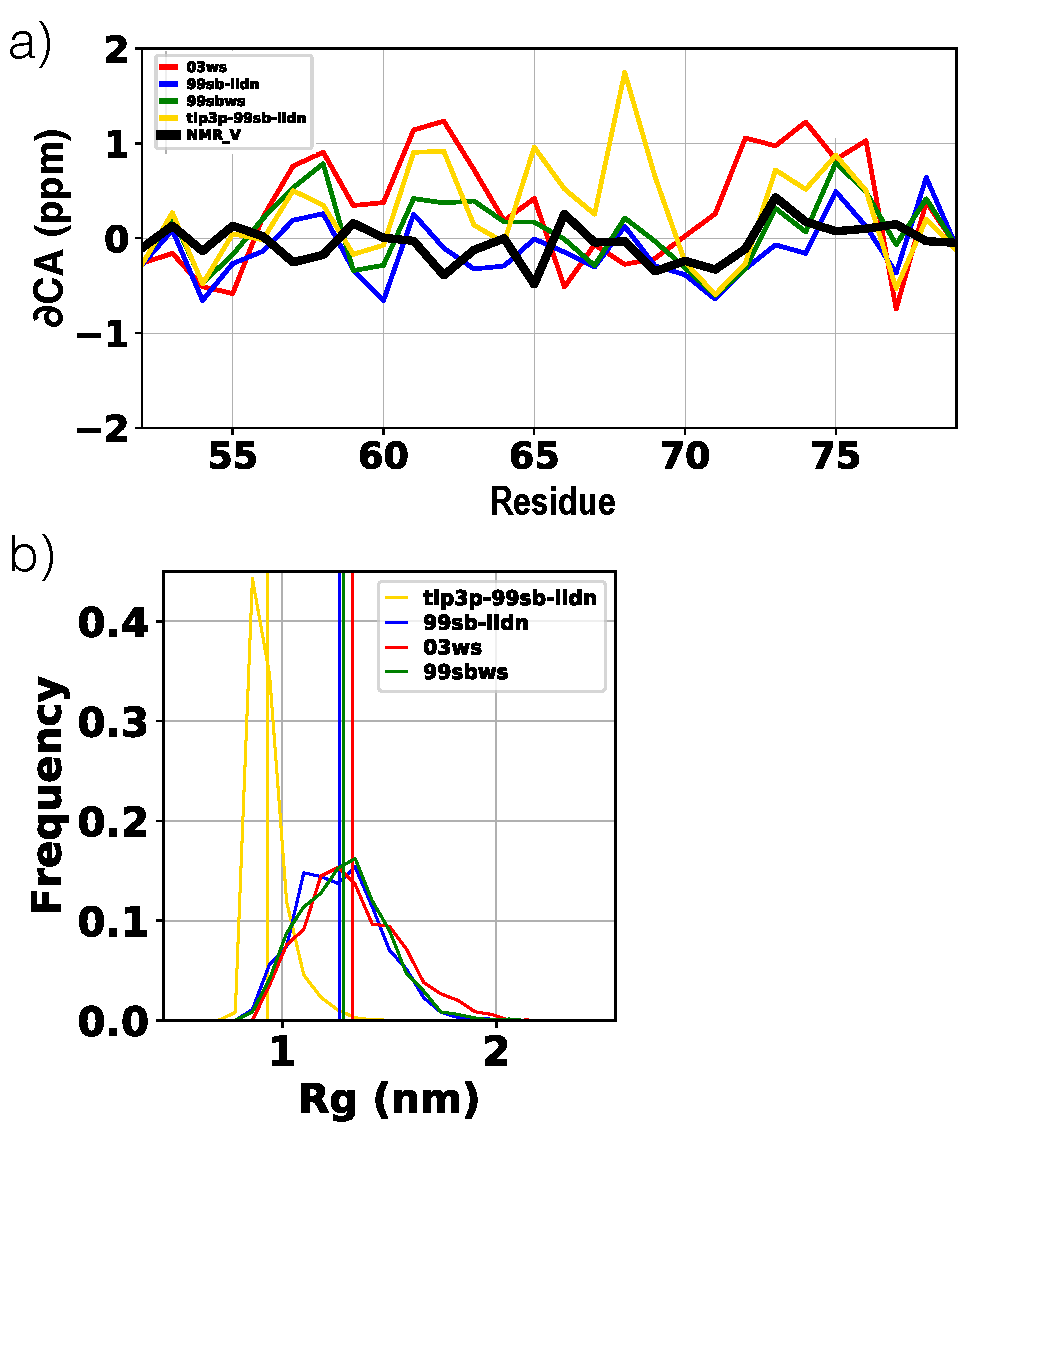
\includegraphics[scale=0.5,width=0.9\textwidth,trim={0 0cm 0 0cm},clip]{../figures/S1.pdf}
\caption{{\bf Force field comparison.} We ran 500ns of T-REMD simulations of a 30 residue fragment of the V66 prodomain with several commonly used force field and water model combinations. The first 200ns of data was discarded as equilibration. (a) Comparison of calculated C\textsubscript{$\alpha$} chemical shifts from MD ensembles at 280K for Amber99sb*-ildn-q~\cite {Lindorff-Larsen2010a, Hornak2006a} with Tip4p-D~\cite{Piana2015} (RMSD 0.36 ppm),  Amber99sbws~\cite{Lindorff-Larsen2010a, Best2014} (RMSD 0.42 ppm), Amberff03sbws~\cite {Best2009, Best2014} (RMSD 0.73 ppm), Amber99sb-ildn with Tip3P ~\cite {Jorgensen1981} (RMSD 0.65 ppm), calculated using SPARTA+~\cite{Shen2010} and NMR C\textsubscript{$\alpha$} chemical shifts (black line) from Ref.~\citenum{Anastasia2013} at 280K. (b) R\textsubscript{g} distribution for each force field. Tip3P generates very collapsed ensembles and the remaining three force field generates similar R\textsubscript{g} distribution. The $\langle R\textsubscript{g} \rangle$ is shown with vertical lines.}
\label{S1} 
\end{figure}


 \begin{figure}[!ht]
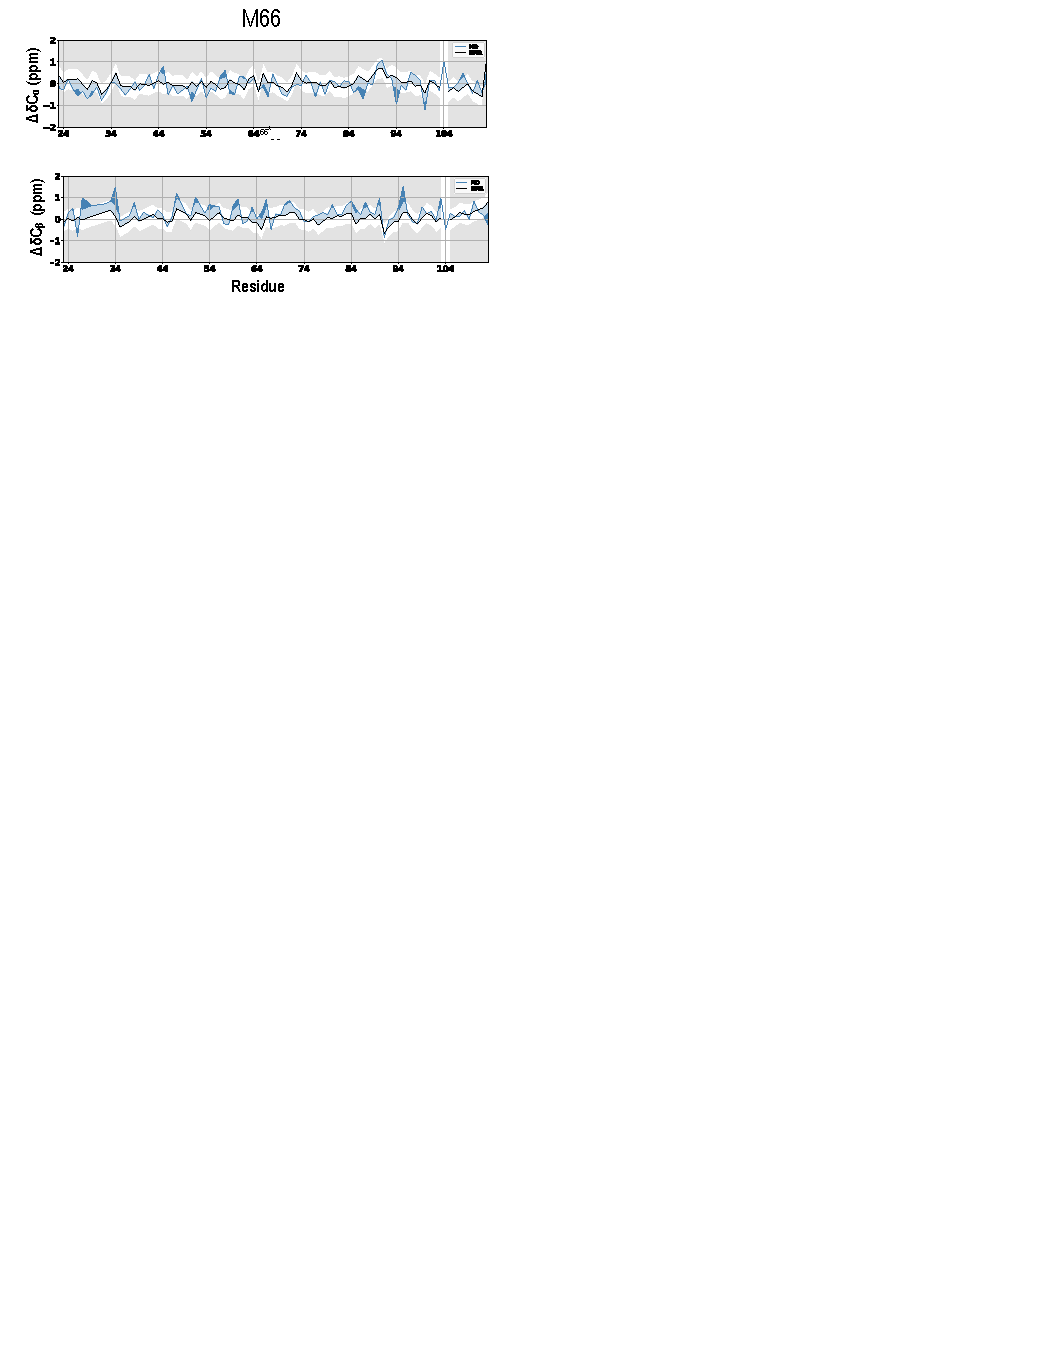
\includegraphics[scale=0.5,width=\textwidth,trim={0 0cm 0 0cm},clip]{../figures/S2.pdf}
\caption{{\bf Comparison of MD and NMR observables.} C\textsubscript{$\alpha$} (top) and C\textsubscript{$\beta$} (bottom) chemical shifts from NMR at 280K (black lines)~\cite{Anastasia2013} and MD at 300K (blue lines), calculated using SPARTA+ ~\cite{Shen2010} for M66 sequence. Chemical shifts outside the range of 0.5 ppm from NMR chemical shifts are shaded grey.}
\label{S2} 
\end{figure}

\begin{figure}[!ht]
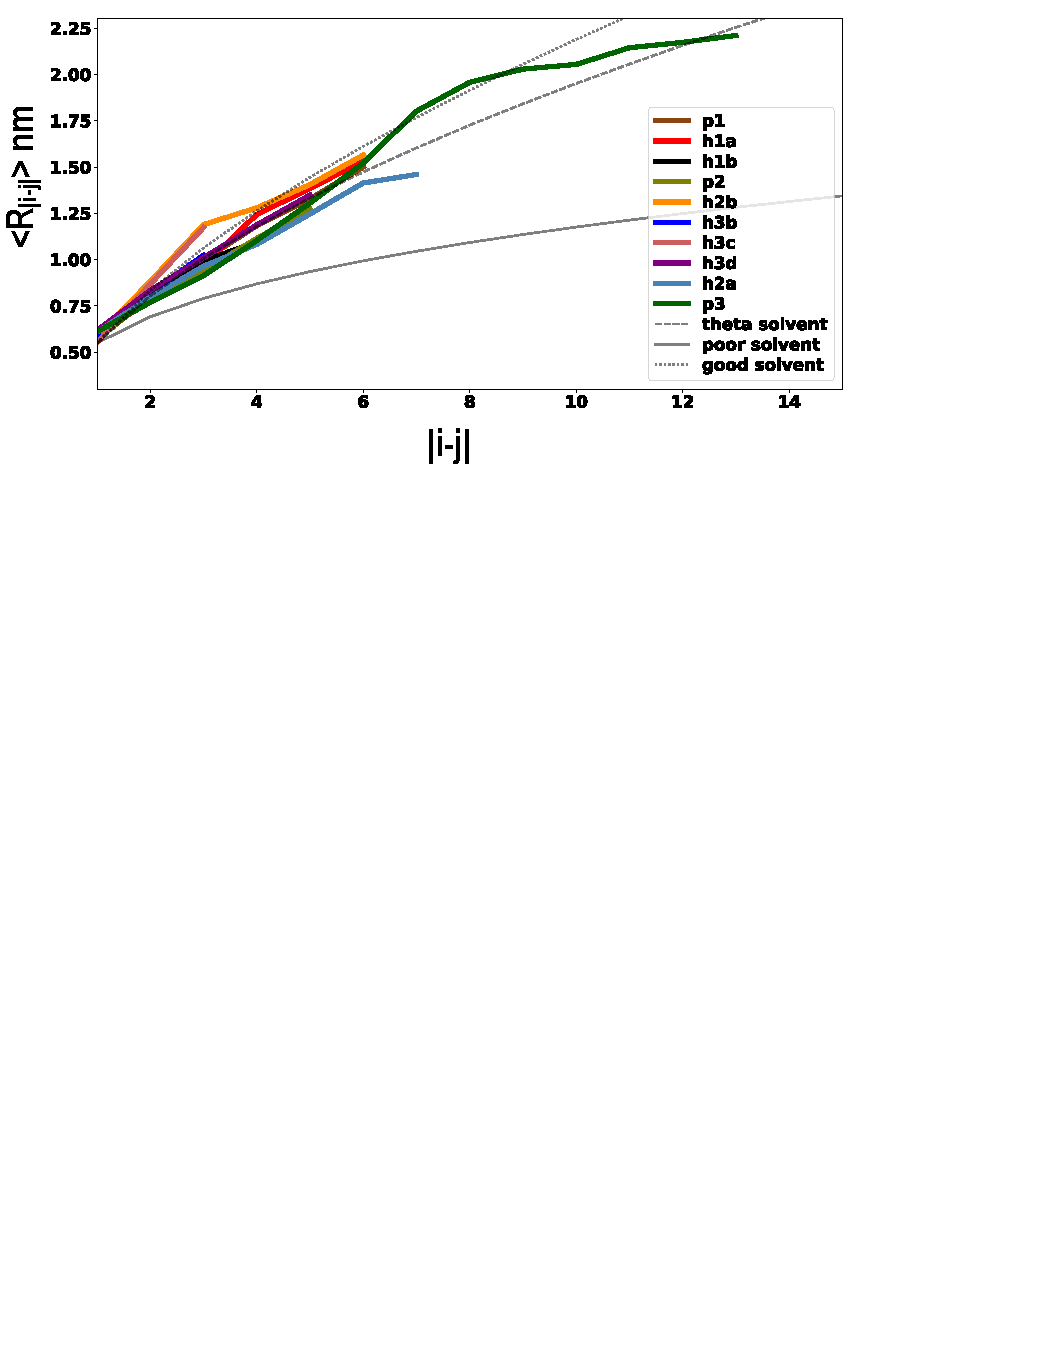
\includegraphics[scale=0.5,width=0.9\textwidth,trim={0 0cm 0 0cm},clip]{../figures/S3.pdf}
\caption{{\bf Scaling behavior of each identified domain.} Ensemble averaged interchain distance profiles for each domain in V66 sequence. Theoretical polymer scaling limits are shown with grey lines (prefactor A = 0.55 nm), while Flory exponents for each curve are given in Table~\ref{t1}. }
\label{S3} 
\end{figure}

\begin{table}[ht]
\caption{Flory exponent ($\nu$) and prefactor (A) for each proregion domain, calculated from MD trajectories. Errors represent fit error of $\langle R_{|i-j|}\rangle$ vs  $A|i-j|^{\nu}$, weighted by each point's standard deviation.}
\label{t1}
\begin{tabular}{|c|c|c|c|c|}
\hline
domain & A (V66)  & $\nu$ (V66) & A (M66)  & $\nu$ (M66)\\          
\hline
p1 &  0.53 $\pm{ 0.16}$ & 0.58 $\pm{ 0.24}$ &  0.52 $\pm{0.15}$ & 0.60 $\pm{0.23}$ \\
\hline
h1a &  0.53 $\pm{ 0.16}$ & 0.59 $\pm{ 0.25}$ &  0.53 $\pm{0.16}$ & 0.60 $\pm{0.24}$ \\
\hline
h1b & 0.61  $\pm{0.24 }$ &0.44  $\pm{0.40 }$ &  0.60 $\pm{0.26}$ & 0.44 $\pm{0.41}$ \\
\hline
p2 & 0.56  $\pm{0.22 }$ &0.50  $\pm{0.34 }$ &  0.59 $\pm{0.18}$ & 0.51 $\pm{0.29}$ \\
\hline
h2a &  0.56 $\pm{ 0.17}$ & 0.50 $\pm{ 0.22}$ &  0.57 $\pm{0.17}$ & 0.48 $\pm{0.23}$ \\
\hline
h2b &  0.64 $\pm{ 0.14}$ & 0.51 $\pm{ 0.18}$ &  0.60 $\pm{0.15}$ & 0.56 $\pm{0.20}$ \\
\hline
p3 &  0.49 $\pm{ 0.09}$ & 0.63 $\pm{ 0.10}$ &  0.50 $\pm{0.09}$ & 0.62 $\pm{0.10}$ \\
\hline
h3b &  0.56 $\pm{ 0.32}$ & 0.55 $\pm{ 0.62}$ &  0.55 $\pm{0.28}$ & 0.60 $\pm{0.57}$ \\
\hline
h3c &  0.52 $\pm{ 0.13}$ & 0.75 $\pm{ 0.29}$ &  0.52 $\pm{0.14}$ & 0.74 $\pm{0.31}$ \\
\hline
h3d & 0.58  $\pm{0.18 }$ &0.52  $\pm{0.27 }$ &  0.59 $\pm{0.19}$ & 0.49 $\pm{0.28}$ \\
\hline
\end{tabular}

\end{table}

 \begin{figure}[!ht]
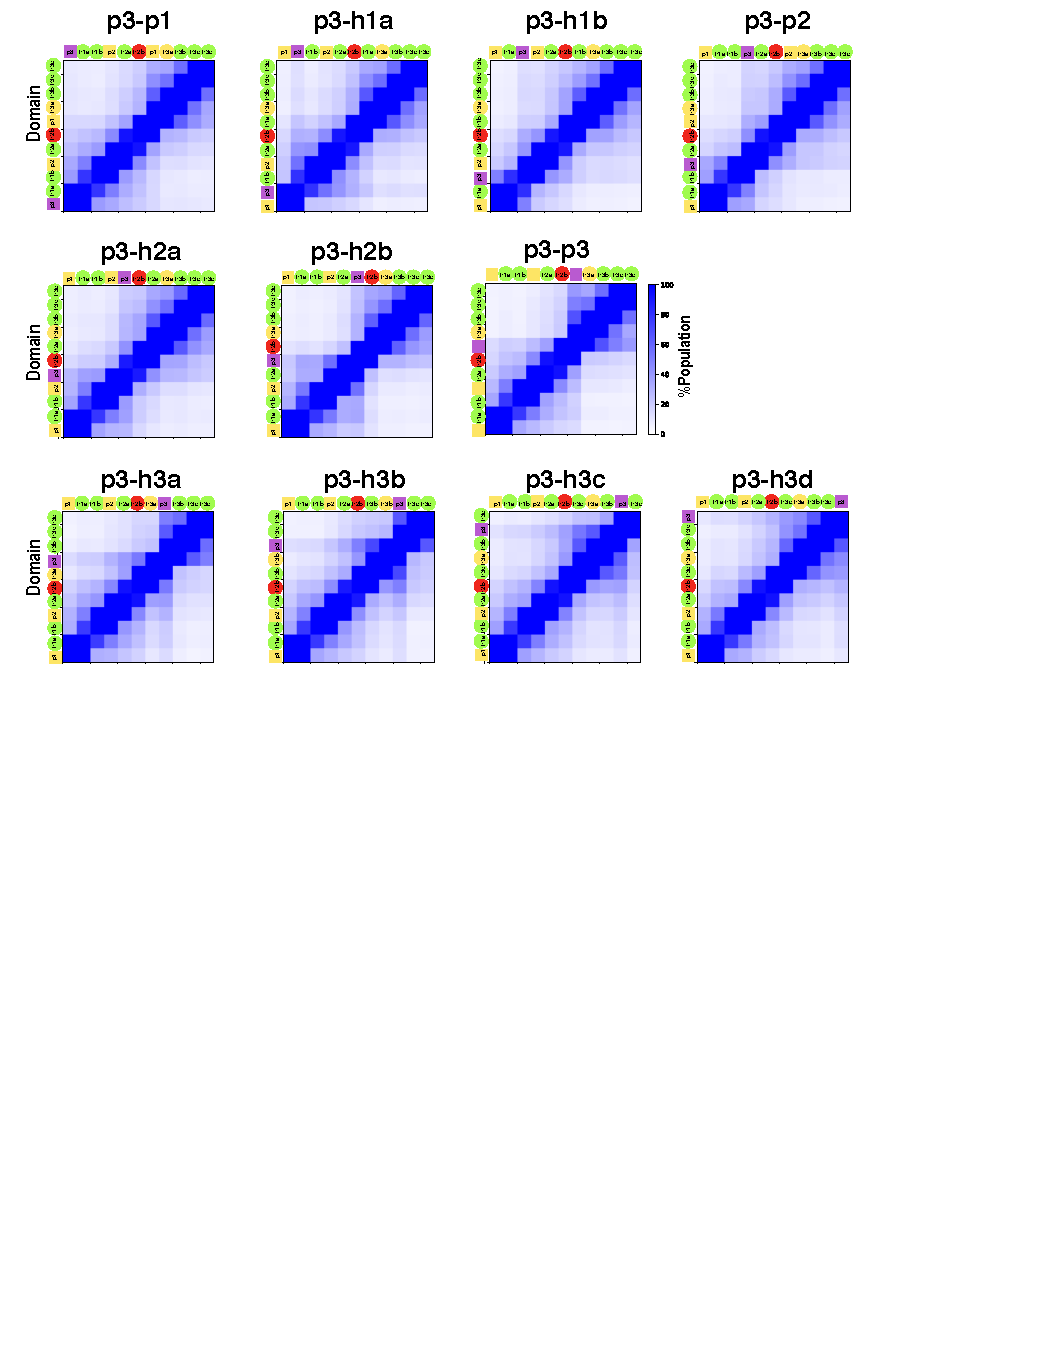
\includegraphics[scale=0.5,width=\textwidth,trim={0 0cm 0 0cm},clip]{../figures/S4.pdf}
\caption{{\bf Effect of perturbing monomer properties on freely-jointed, self-avoiding heteropolymer} Contact probability maps from MC simulations, analogous to those in Figure 3 of the main text, in which the monomer with properties of linker domain p3 is swapped with every other monomer on the chain, with the new location represented by the purple square in the graph annotation.  As the p3 bead is shifted along the chain, p3 and p1 consistently bound a white ``forbidden'' region that has little interaction with the rest of the protein. }
\label{S4} 
\end{figure}



\begin{figure}[!ht]
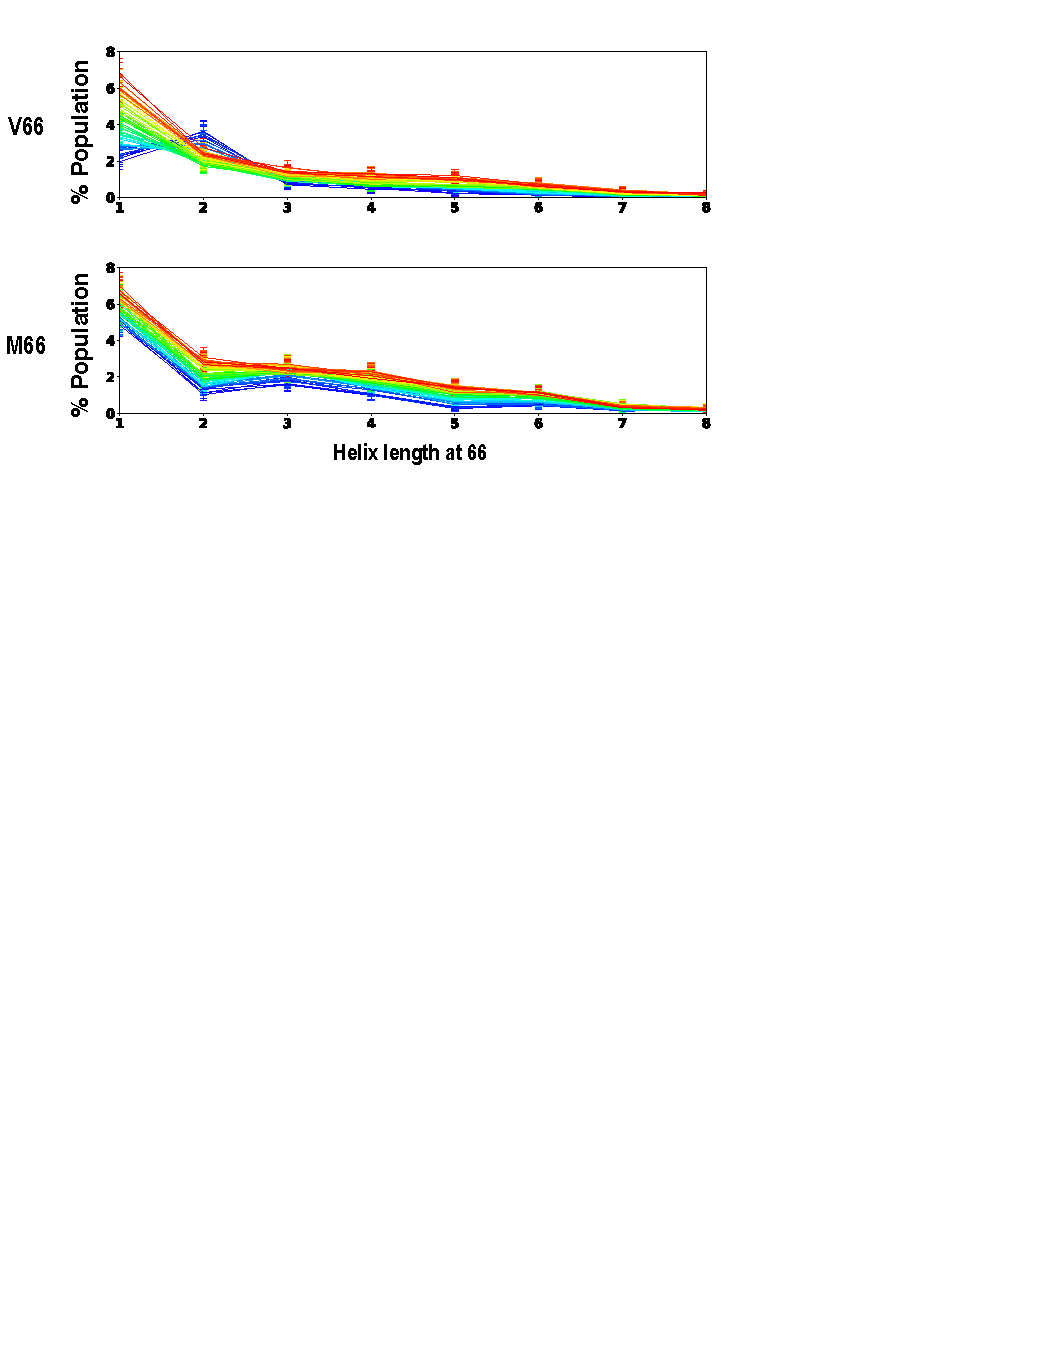
\includegraphics[scale=0.5,width=0.9\textwidth,trim={0 0cm 0 0cm},clip]{../figures/S6.pdf}
\caption{{\bf Effects of temperature and Val66Met mutation on helix propensity around residue 66.} Frequency of helix of a given length at residue 66 in V66 (top) and M66 (bottom) in the temperature range of 300K to 385 K. With the increase in temperature the color transitions from cooler (blue) to hotter (red).  It is entropically unfavorable for V66 and its neighboring residue to be simultaneously in the helical region of the Ramachandran map, as indicated by the decreasing helical propensity with increasing temperature.  For longer helices, the trend will depend more on the additional side-chains in the helix, and the trend with temperature is reversed, but it remains weaker than the analogous trend for the M66 sequence.  Errors represent standard error of a Bernoulli trial with n number of samples, where n is the product of total number unique replicas forming the helix of given length at residue 66 at a given temperature and average number of roundtrips per replica, 17.}
\label{S5} 
\end{figure}

 \begin{figure}[!ht]
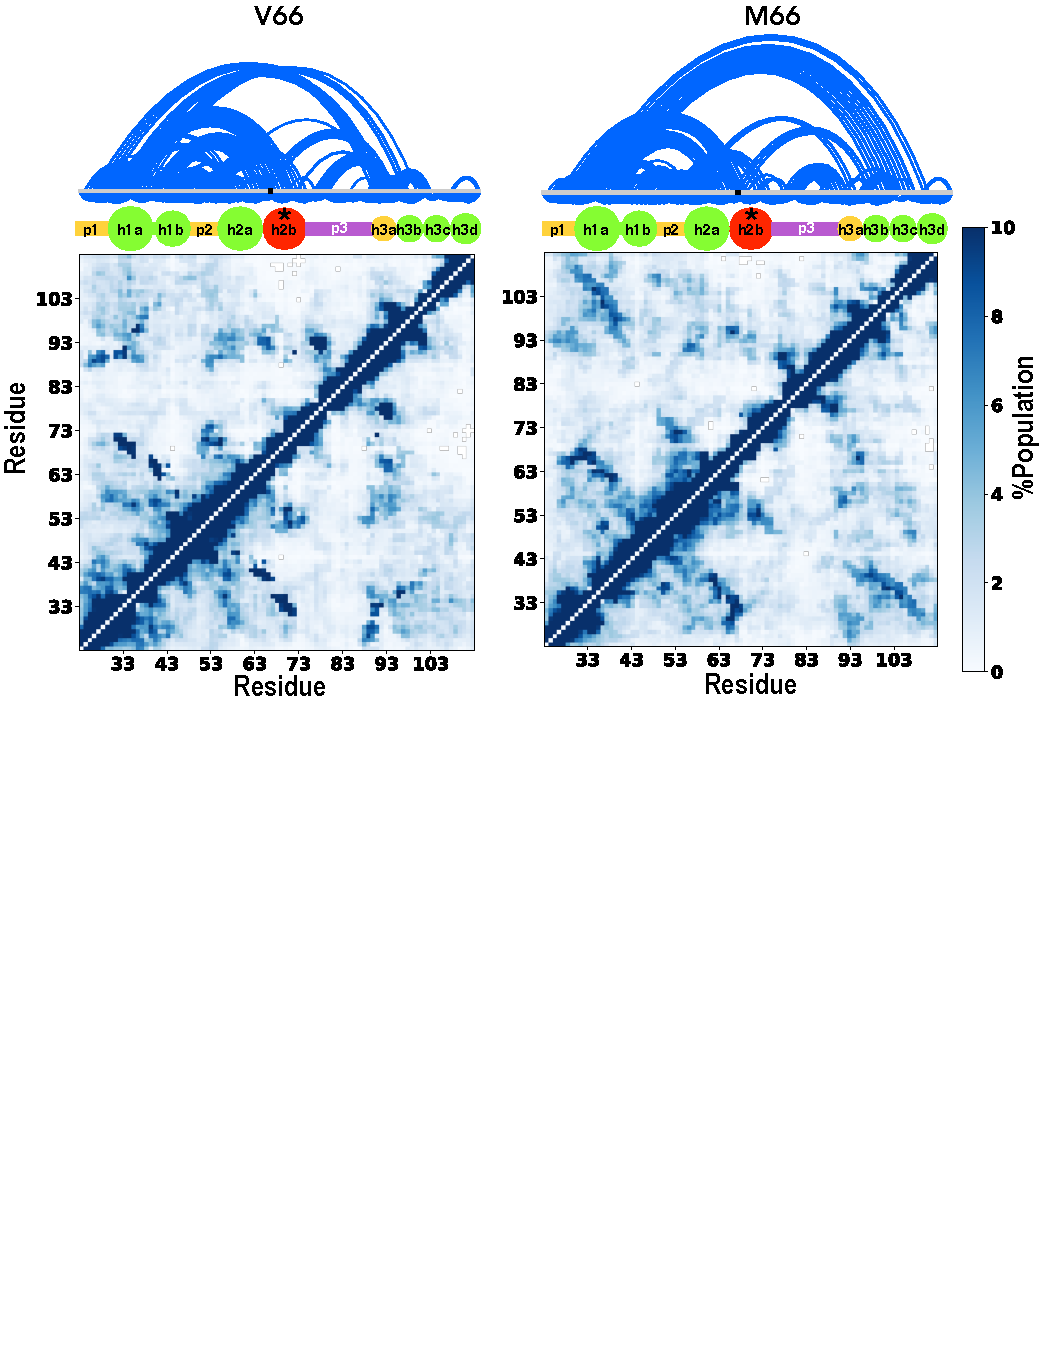
\includegraphics[scale=0.5,width=\textwidth,trim={0 0cm 0 0cm},clip]{../figures/S5.pdf}
\caption{{\bf Residue level contacts for the entire prodomain.} Contact probability between every residue pair for V66 (left) and M66 (right). A linear network of transient tertiary contacts is also shown (top) for each form. Two residue pairs are in contact if the distance between C\textsubscript{$\alpha$}-C\textsubscript{$\alpha$} atoms between the two residues are 0.8nm or less. The contact networks were build using Cytoscape~\cite{Ahlstrom2013} with a linear representation of residues. Each protein residue comprises a node in the network, with interactions between residues represented as edges. The strength of individual interactions can be interpreted by the thickness of the edge line on the network diagram. If the separation between residues forming the contact is more than 3, its edge is drawn above the node; otherwise, the edge is drawn at the bottom of the node. To focus on significant interactions, interactions showing more than 4\% persistence were considered in network visualization.}
\label{S6} 
\end{figure}

\begin{figure}[!ht]
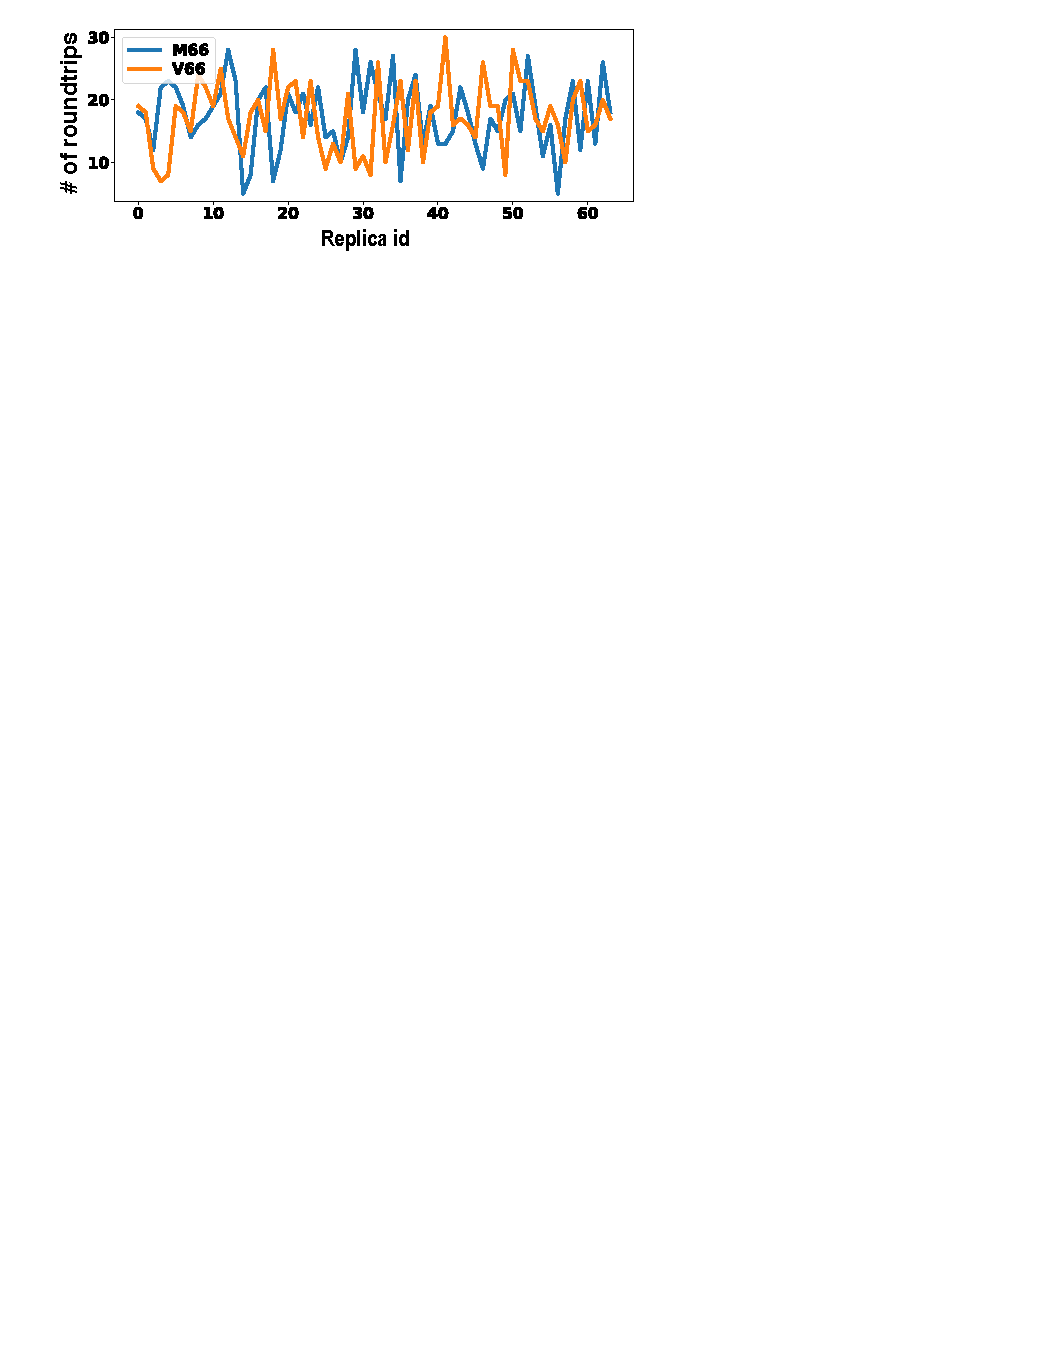
\includegraphics[scale=0.5,width=0.9\textwidth,trim={0 0cm 0 0cm},clip]{../figures/S7.pdf}
\caption{{\bf Number of round trip completed by each replica.} Both V66 and M66 complete a minimum 5 roundtrips for each replica and an average of 17 round-tips per replica over the course of 76.8 $\mu$s (1.2 $\mu$s $\times$64) of simulations.}
\label{S7} 
\end{figure}

\clearpage

\bibliography{IDP_Val66Met_Lohia}

\end{document}

